\documentclass[12pt,a4paper]{article}

\usepackage{float}
\usepackage{cmap}
\usepackage[T1]{fontenc}
\usepackage[utf8x]{inputenc}
\usepackage{amssymb}
\usepackage{amsmath}
\usepackage[danish]{babel}
\usepackage{graphicx}
\usepackage{hyperref}
\usepackage[all]{hypcap}
\hypersetup{
    colorlinks=true,
    linkcolor=blue,
    filecolor=magenta,      
    urlcolor=cyan,
    pdftitle={1g første ugeopgave},
    pdfpagemode=FullScreen,
    }

\urlstyle{same}

\title{PoP -- ugeopgave 2}
\author {Sofus Ostrowska Bjørn \texttt{<dxq257>}}
\date{\today}

\begin{document}

\maketitle

\section*{2i0}
Et Fsharp program kan køres på tre forskellige måder fra terminalen.   
\begin{itemize}
    \item Gennem et 'interactive session' (\textit{fsharpi} og ;;)
    \item Ved at interprete en  skrevet .fsx fil, også igennem\textit{ fsharpi} (;; er ikke nødvendige her)
    \item Til sidst ved kan man køre det ved at compile en .fsx fil, med \textit{fsharpc} og dernæst køre den skapte .exe med mono
\end{itemize}
Det viser sig at det i første omgang er hurtigere at interprete en .fsx fil; \textbf{Men det gælder kun hvis man kører det én enkel gang}. Det vil altid være hurtigere at compile det, og dernæst køre .exe'en i mono, hvis man har tænkt sig at gøre det mere end én gang.
Jeg tænker at en interactive session er god til at, i første omgang, at få en forståelse for fsharp og hvordan det virker. I anden omgang er det velsagtens smart at køre små script-fragments i en interactive session, da man kan gøre det hele inden i terminalen og får direkte svar, samt fejlkoder, hvis noget ikke var korrekt.

\section*{2i1}
Siden jeg ikke har kunne læse mig frem til noget omkring 'slicing', i hvert fald når det kommer til strings, har jeg valgt at benytte \textit{dot-notation} til at 'splice' min string 'Hello World'.
Jeg startede med at få en masse errors for at bruge de forkerte citationstegn til mit string... som åbenbart er anderledes i aquamacs end de er i terminalen.
Dernæst erfarrede jeg at der ikke var noget output, så min plan er at få printfn til at virke med min string.
\begin{figure}[H]
    \centering
    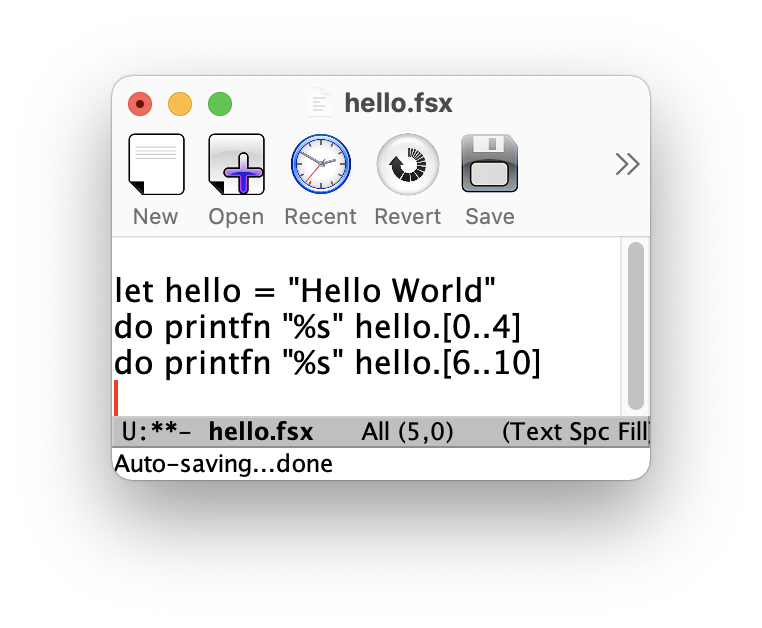
\includegraphics[width=0.5\linewidth]{Aqua.png}
    \caption{Her ses den expression jeg har valgt til at splice min string}
    \label{fig:1}
\end{figure}
\begin{figure}[H]
    \centering
    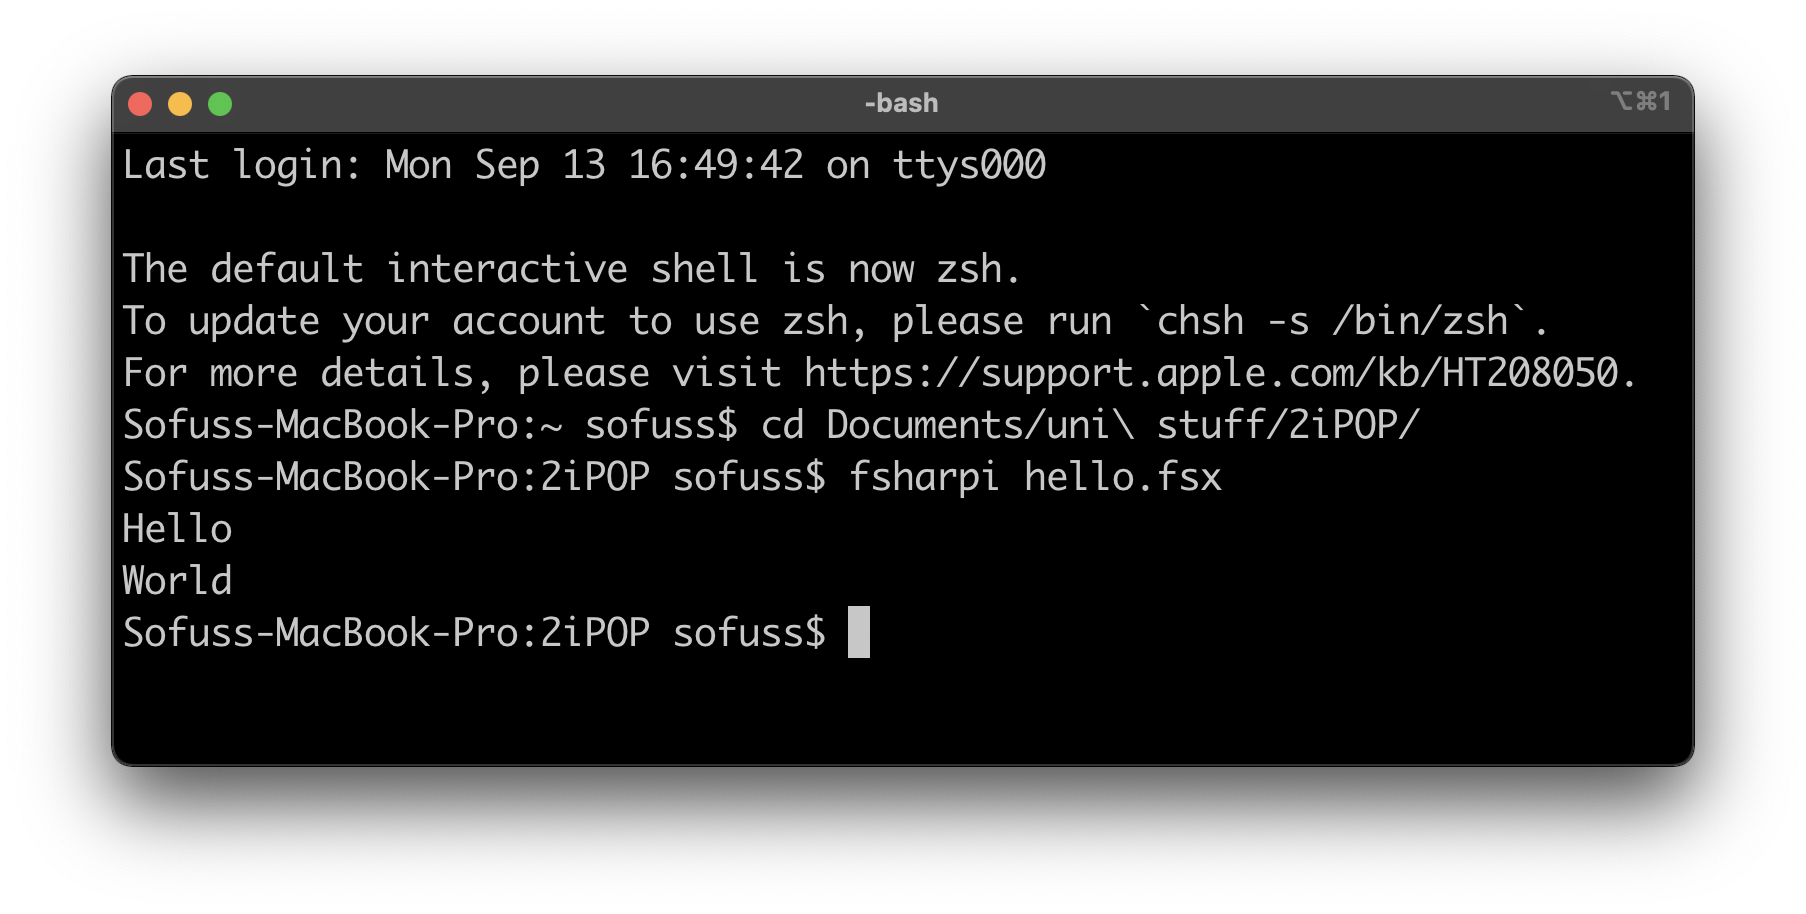
\includegraphics[width=0.5\linewidth]{Term.png}
    \caption{Her ses hvordan min .fsx fil bliver interpreted, og at programmet har outputtet: 'Hello', 'World'}
    \label{fig:2}
\end{figure}

\section*{2i2}

Opgaven er lavet i hånden og senere indsat i latex på stråelende vis.
\begin{table}[H]
\begin{center}
\begin{tabular}{|c|c|c|c|}
\hline
Decimal & Binary & Hexadecimal & Octal \\ \hline
10      & 1010   & a           & 12    \\ \hline
21      & 10101  & 15          & 25    \\ \hline
47      & 101111 & 2f          & 57    \\ \hline
59      & 111011 & 3b          & 73    \\ \hline
\end{tabular}
\end{center}
\end{table}

Her medfølger mellemregninger for følgende:\\
\noindent Decimal to binary for 10\textsubscript{10}: 
\begin{align}
\centering
10/2 = 5, && 10\%2 &= 0 \\
5/2 = 2, && 5\%2 &= 1 \\
2/2 = 1, && 2\%2 &= 0 \\
1/2 = 0, && 1\%2 &= 1 \\
&& 10_{10}&= 1010_{2}
\end{align}
\noindent Binary to decimal for 10101\textsubscript{2}: 
\begin{align}
1*2^0&=1\\
1*2^2&=4\\
1*2^4&=16 \\
1+4+16&=21 \\
10101_{2} &= 21_{10}
\end{align}
\noindent Binary to hexadecimal for 1010\textsubscript{2}: 
\begin{align}
1010_{2}=10_{10}&=a_{16}\\
\end{align}
\noindent Hexadecimal to binary for 2f\textsubscript{16}: 
\begin{align}
2_{16}&=0010_{2}\\
f_{16}&=1111_{2}\\
2f_{16} = 00101111_{2}&= 101111_{2}
\end{align}
\noindent Binary to octal for (0)10101\textsubscript{2}: 
\begin{align}
010_{2}&=2_{8}\\
101_{2}&=5_{8}\\
10101_{2} &= 25_{8}
\end{align}
\noindent Octal to binary for 73\textsubscript{8}: 
\begin{align}
7_{8}&=1110_{2}\\
3_{8}&=11_{2}\\
73_{8}&= 111011_{2}
\end{align}

\end{document}